
\begin{frame}[t]
\frametitle{course material: Learn Prolog Now!}


\textbf{Aim of the course}: to advertise Prolog via programming in it.\\

\[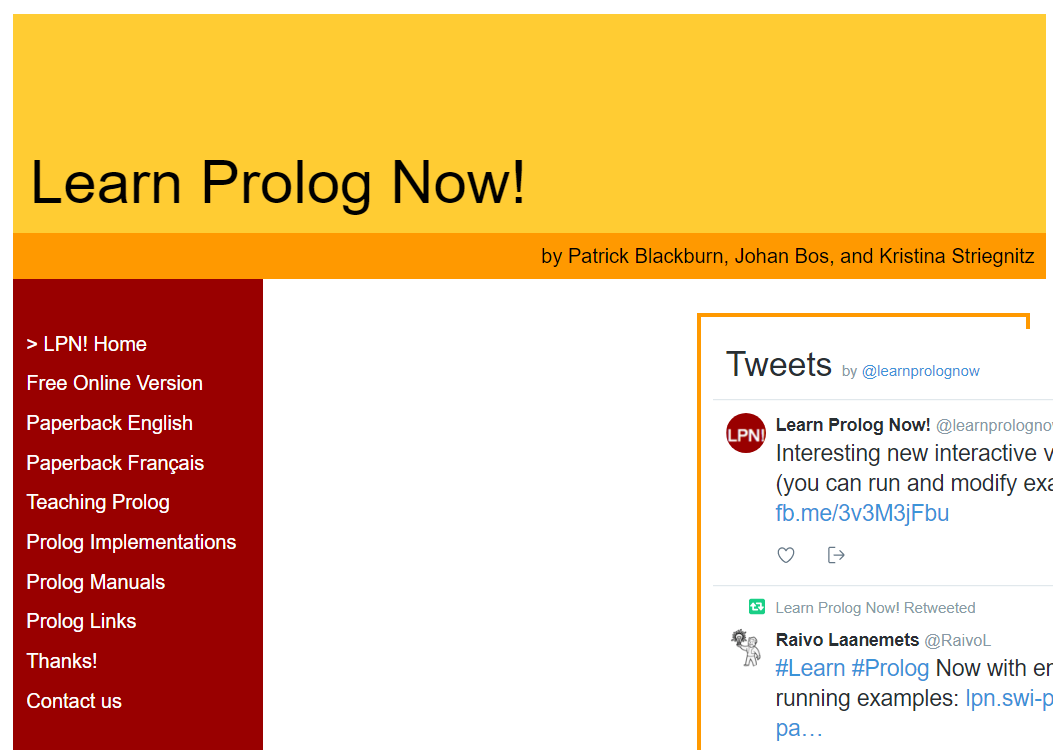
\includegraphics[width=.5\textwidth]{LPNwebsite.png}
\quad 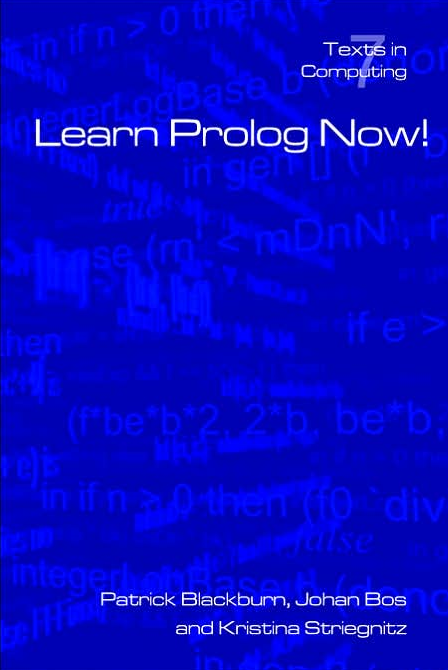
\includegraphics[width=.25\textwidth]{lpncover.png}
\]

One of the best introductory books. It does not cover much, but it is an excellent introduction \textbf{written by logicians}.

\vfill \hfill
(for modal logicians: one of the authors is Patrick Blackburn!)

\end{frame}


\begin{frame}[t]
\frametitle{Outline}

Introduction (history, basic concepts, course material)
\begin{itemize}
\item history
\item basic concepts
\item course material
\end{itemize}
\bigskip

Syntax
\begin{itemize}
\item elements of the language
\item facts, rules, knowledge base
\item queries
\end{itemize}
\bigskip

Horn clauses
\bigskip

Unification

	\begin{tikzpicture}
\node[overlay, rotate = -90] at (7.7,6.35){
\includegraphics[scale=.17]{prologlogo.png}};
\end{tikzpicture}
\end{frame}
